\documentclass[12pt,onecolumn]{article}
\usepackage[utf8]{inputenc} % UTF8 input encoding
\usepackage[T2A]{fontenc}   % T2A font encoding for Cyrillic script
\usepackage[russian]{babel} % Russian language support
\usepackage{listings}
\usepackage{tikz}
\usepackage{float}
\usepackage{mathtools}
\everymath{\displaystyle}
\usepackage{hyperref}
\usepackage[table,xcdraw]{xcolor}
\usepackage{geometry}
\usepackage{verbatim}
\usepackage{pdfpages}
\usepackage{graphicx}
\usepackage{url}
\newcommand{\nparagraph}[1]{\paragraph{#1}\mbox{}\\}
\geometry{
  a4paper,
  top=20mm, 
  right=20mm, 
  bottom=20mm, 
  left=25mm
}
\lstdefinestyle{verilog}{ 
  basicstyle=\small\ttfamily,
  commentstyle=\color{cyan},
  stringstyle=\color{magenta}\ttfamily,
  keywordstyle=\color{blue},
  numbers=left,
  numberstyle=\scriptsize,
  numbersep=5pt,
  frame=single,
  breaklines=true,
  breakatwhitespace=true,
  showstringspaces=false,
  tabsize=4,
  inputencoding=utf8,
  extendedchars=true
}

\begin{document}
\setcounter{tocdepth}{4}
\begin{center}
  Федеральное государственное автономное образовательное учреждение высшего образования "Национальный Исследовательский Университет ИТМО"\\
  Мегафакультет Компьютерных Технологий и Управления\\
  Факультет Программной Инженерии и Компьютерной Техники \\
  
\includegraphics[scale=0.3]{image/itmo.jpg} % нужно закинуть картинку логтипа в папку с отчетом
\end{center}
\vspace{1cm}


\begin{center}
  \textbf{Лабораторная работа 4}\\
  по дисциплине\\
  \textbf{Тестирование программного обеспечения}
\end{center}

\vspace{2cm}

\begin{flushright}
  Выполнил Студент  группы P33102\\
  \textbf{Лапин Алексей Александрович}\\
  Преподаватель: \\
  \textbf{Харитонова Анастасия Евгеньевна}\\
\end{flushright}

\vspace{9cm}
\begin{center}
  г. Санкт-Петербург\\
  2024г.
\end{center}
\pagestyle{empty}
\newpage
\section*{Текст задания:}

С помощью программного пакета Apache JMeter провести нагрузочное и\\ стресс-тестирование веб-приложения в соответствии с вариантом задания.

В ходе нагрузочного тестирования необходимо протестировать 3 конфигурации аппаратного обеспечения и выбрать среди них наиболее дешёвую, удовлетворяющую требованиям по максимальному времени отклика приложения при заданной нагрузке (в соответствии с вариантом).

В ходе стресс-тестирования необходимо определить, при какой нагрузке выбранная на предыдущем шаге конфигурация перестаёт удовлетворять требованиями по максимальному времени отклика. Для этого необходимо построить график зависимости времени отклика приложения от нагрузки.


\begin{center}
  \fbox{
    \begin{minipage}{\textwidth}
      Приложение для тестирования доступно только во внутренней сети кафедры.
    \end{minipage}
  }
\end{center}


\begin{center}
  \fbox{
    \begin{minipage}{\textwidth}
      Если запрос содержит некорректные параметры, сервер возвращает HTTP 403.
    \end{minipage}
  }
\end{center}


\begin{center}
  \fbox{
    \begin{minipage}{\textwidth}
      Если приложение не справляется с нагрузкой, сервер возвращает HTTP 503.
    \end{minipage}
  }
\end{center}

\textbf{Параметры тестируемого веб-приложения:}
\begin{enumerate}
  \item URL первой конфигурации (\$ 5100) - \url{http://stload.se.ifmo.ru:8080?token=492469458&user=2109740789&config=1};
  \item URL второй конфигурации (\$ 8400) - \url{http://stload.se.ifmo.ru:8080?token=492469458&user=2109740789&config=2};
  \item URL третьей конфигурации (\$ 16200) - \url{http://stload.se.ifmo.ru:8080?token=492469458&user=2109740789&config=3};
  \item Максимальное количество параллельных пользователей - 14;
  \item Средняя нагрузка, формируемая одним пользователем - 20 запр. в мин.;
  \item Максимально допустимое время обработки запроса - 920 мс.
\end{enumerate}
\textbf{Отчёт по работе должен содержать:}
\begin{enumerate}
  \item Текст задания.
  \item Описание конфигурации JMeter для нагрузочного тестирования.
  \item Графики пропускной способности приложения, полученные в ходе нагрузочного тестирования.
  \item Выводы по выбранной конфигурации аппаратного обеспечения.
  \item Описание конфигурации JMeter для стресс-тестирования.
  \item График изменения времени отклика от нагрузки для выбранной конфигурации, полученный в ходе стресс-тестирования системы.
  \item Выводы по работе.
\end{enumerate}

\section*{Описание конфигурации JMeter для нагрузочного тестирования.}

\begin{figure}[H]
  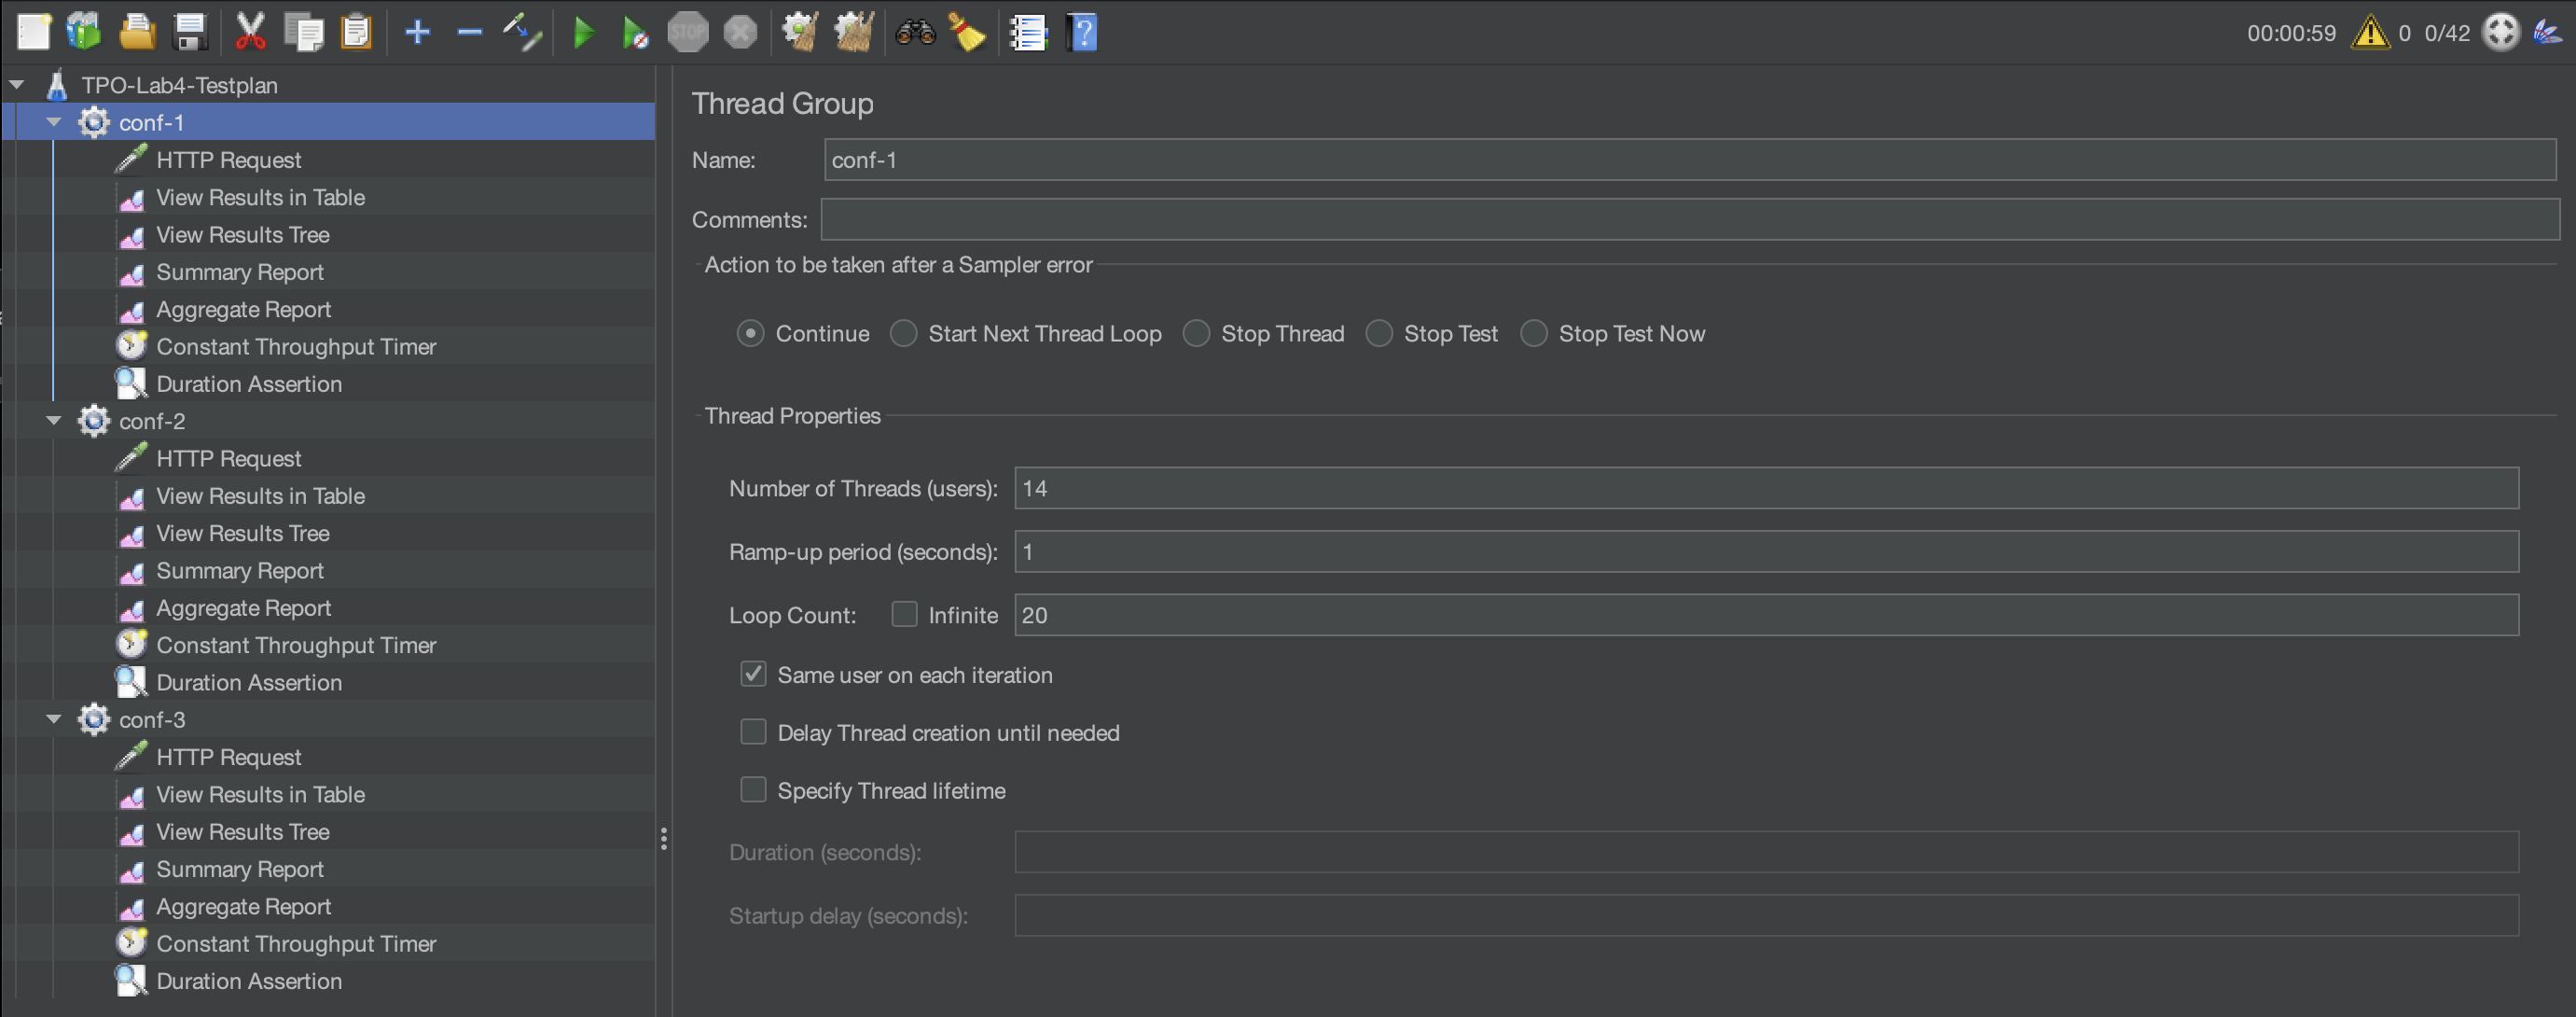
\includegraphics[width=\textwidth]{image/thread-group.png}
  \caption{Вид конфигурации для нагрузочного тестирования}
\end{figure}

Задал конфигурацию для Thread Group:
\begin{itemize}
  \item[] Number of Threads (число пользователей): 14
  \item[] Ramp-Up Period (время нарастания нагрузки): 1 сек.
  \item[] Loop Count (количество итераций): 20 запросов
\end{itemize}

\begin{figure}[H]
  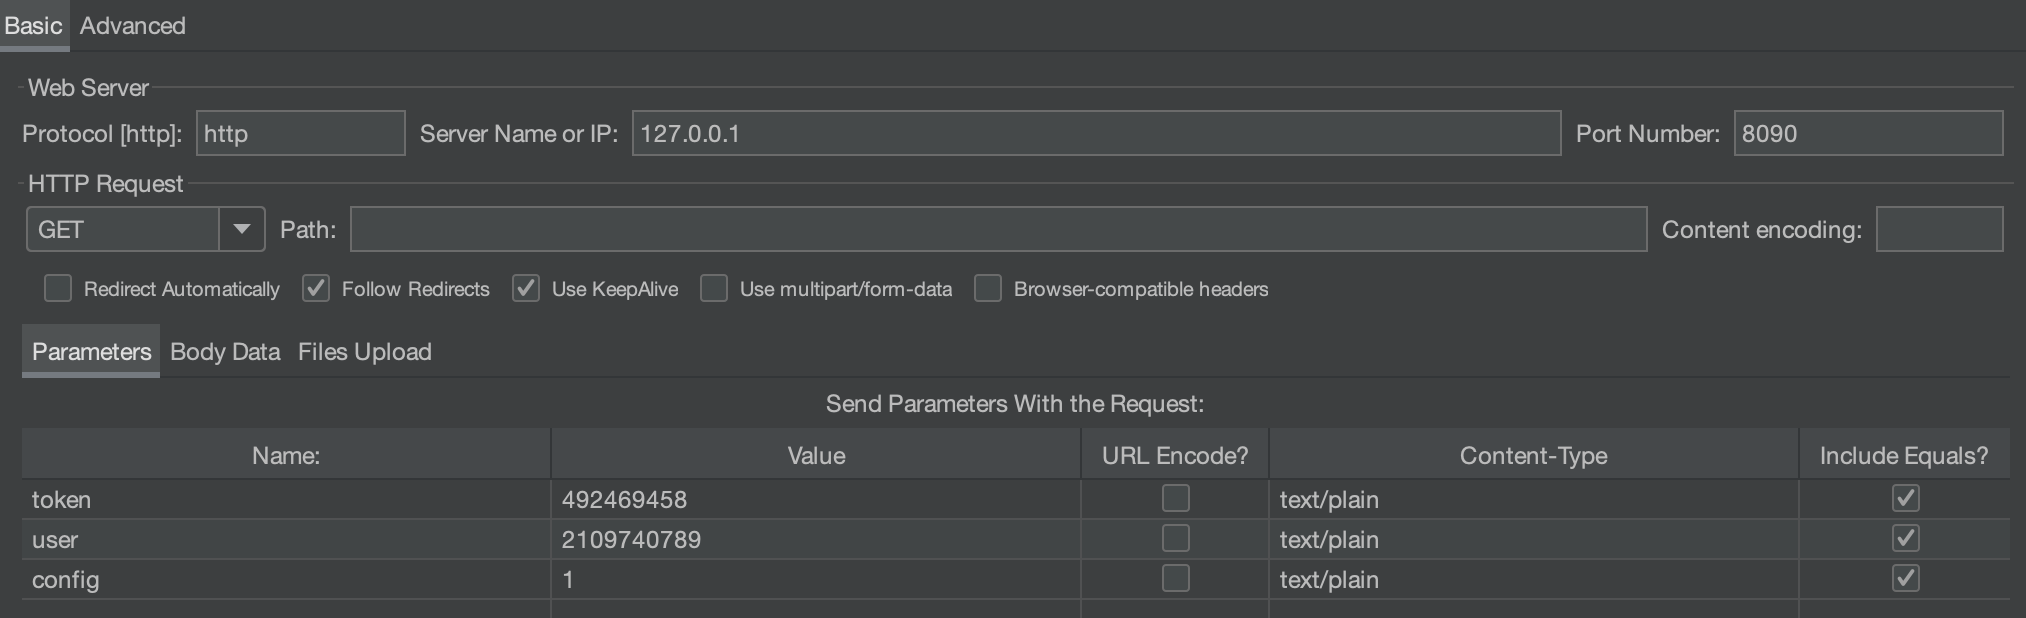
\includegraphics[width=\textwidth]{image/http-request.png}
  \caption{Вид конфигурации для HTTP Request}
\end{figure}

Задал конфигурацию для HTTP Request соответсвенно варианту задания:
\begin{itemize}
  \item[] Protocol: HTTP
  \item[] Server Name or IP: stload.se.ifmo.ru
  \item[] Port Number: 8090
  \item[] Method: GET
  \item[] Parameters: token=492469458\&user=2109740789\&config=1
\end{itemize}

\begin{figure}[H]
  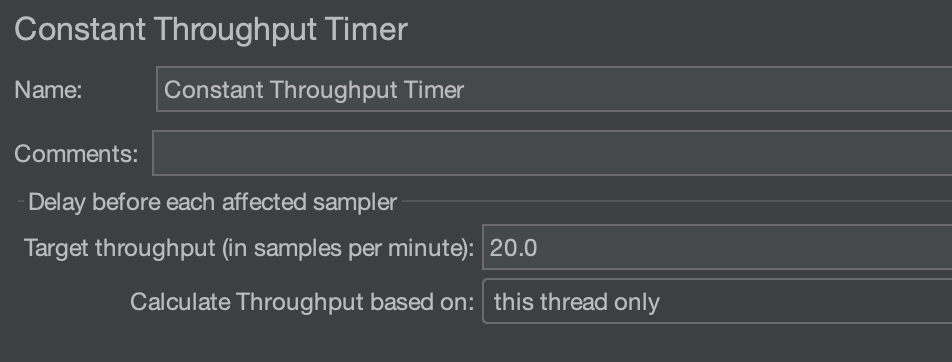
\includegraphics[width=\textwidth]{image/constant-throughput-timer.png}
  \caption{Вид конфигурации для Constant Throughput Timer}
\end{figure}

Задал конфигурацию для Constant Throughput Timer:
\begin{itemize}
  \item[] Target Throughput (запросов в минуту) на одного пользователя: 20
\end{itemize}

\begin{figure}[H]
  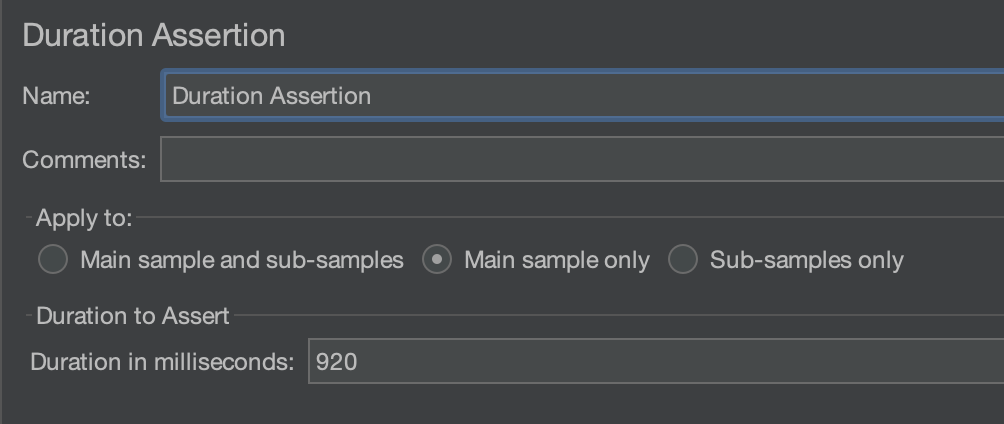
\includegraphics[width=\textwidth]{image/duration-assertion.png}
  \caption{Вид конфигурации для Duration Assertion}
\end{figure}

Задал конфигурацию для Duration Assertion:
\begin{itemize}
  \item[] Максимально допустимое время обработки запроса: 920 мс
\end{itemize}

Повторил настройки для двух других конфигураций.

\section*{Графики пропускной способности приложения, полученные в ходе нагрузочного тестирования.}

Тестовые сценарии запускались как по отдельности, disable/enable для thread-
групп для их выключения и включения, так и все вместе.
Таким образом было получено, что результаты при запуске конфигураций
параллельно отличаются незаметно.

Так как после 1000 семплов сервер начинает заметно снижать скорость ответа.
Будем тестировать до 700 семплов.

\section*{Выводы по выбранной конфигурации аппаратного обеспечения.}

\begin{figure}[H]
  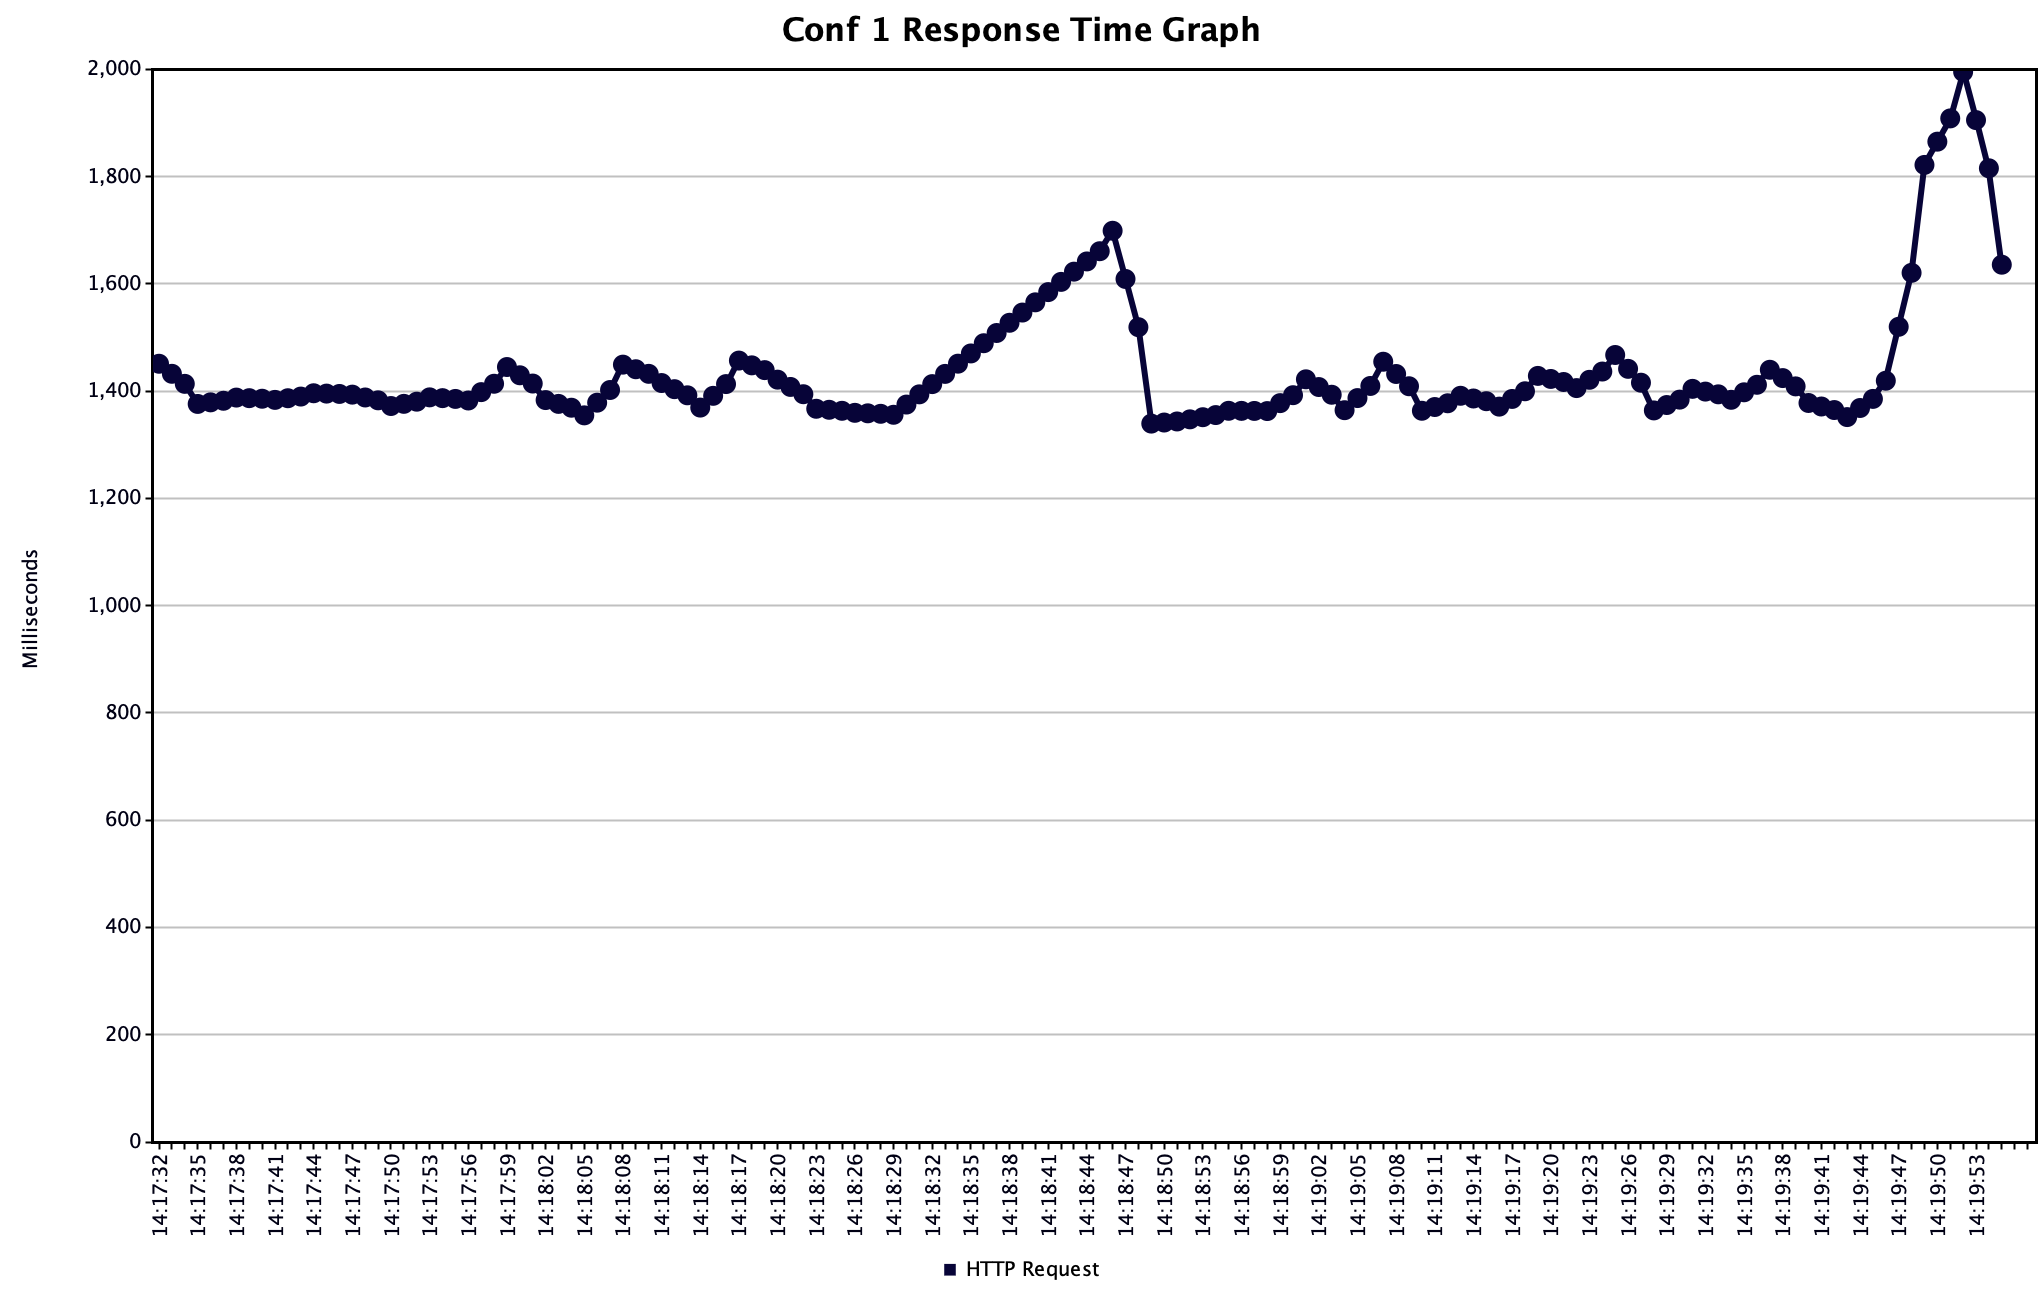
\includegraphics[width=\textwidth]{image/resp-graph-conf-1.png}
  \caption{График пропускной способности для конфигурации 1}
\end{figure}

\begin{figure}[H]
  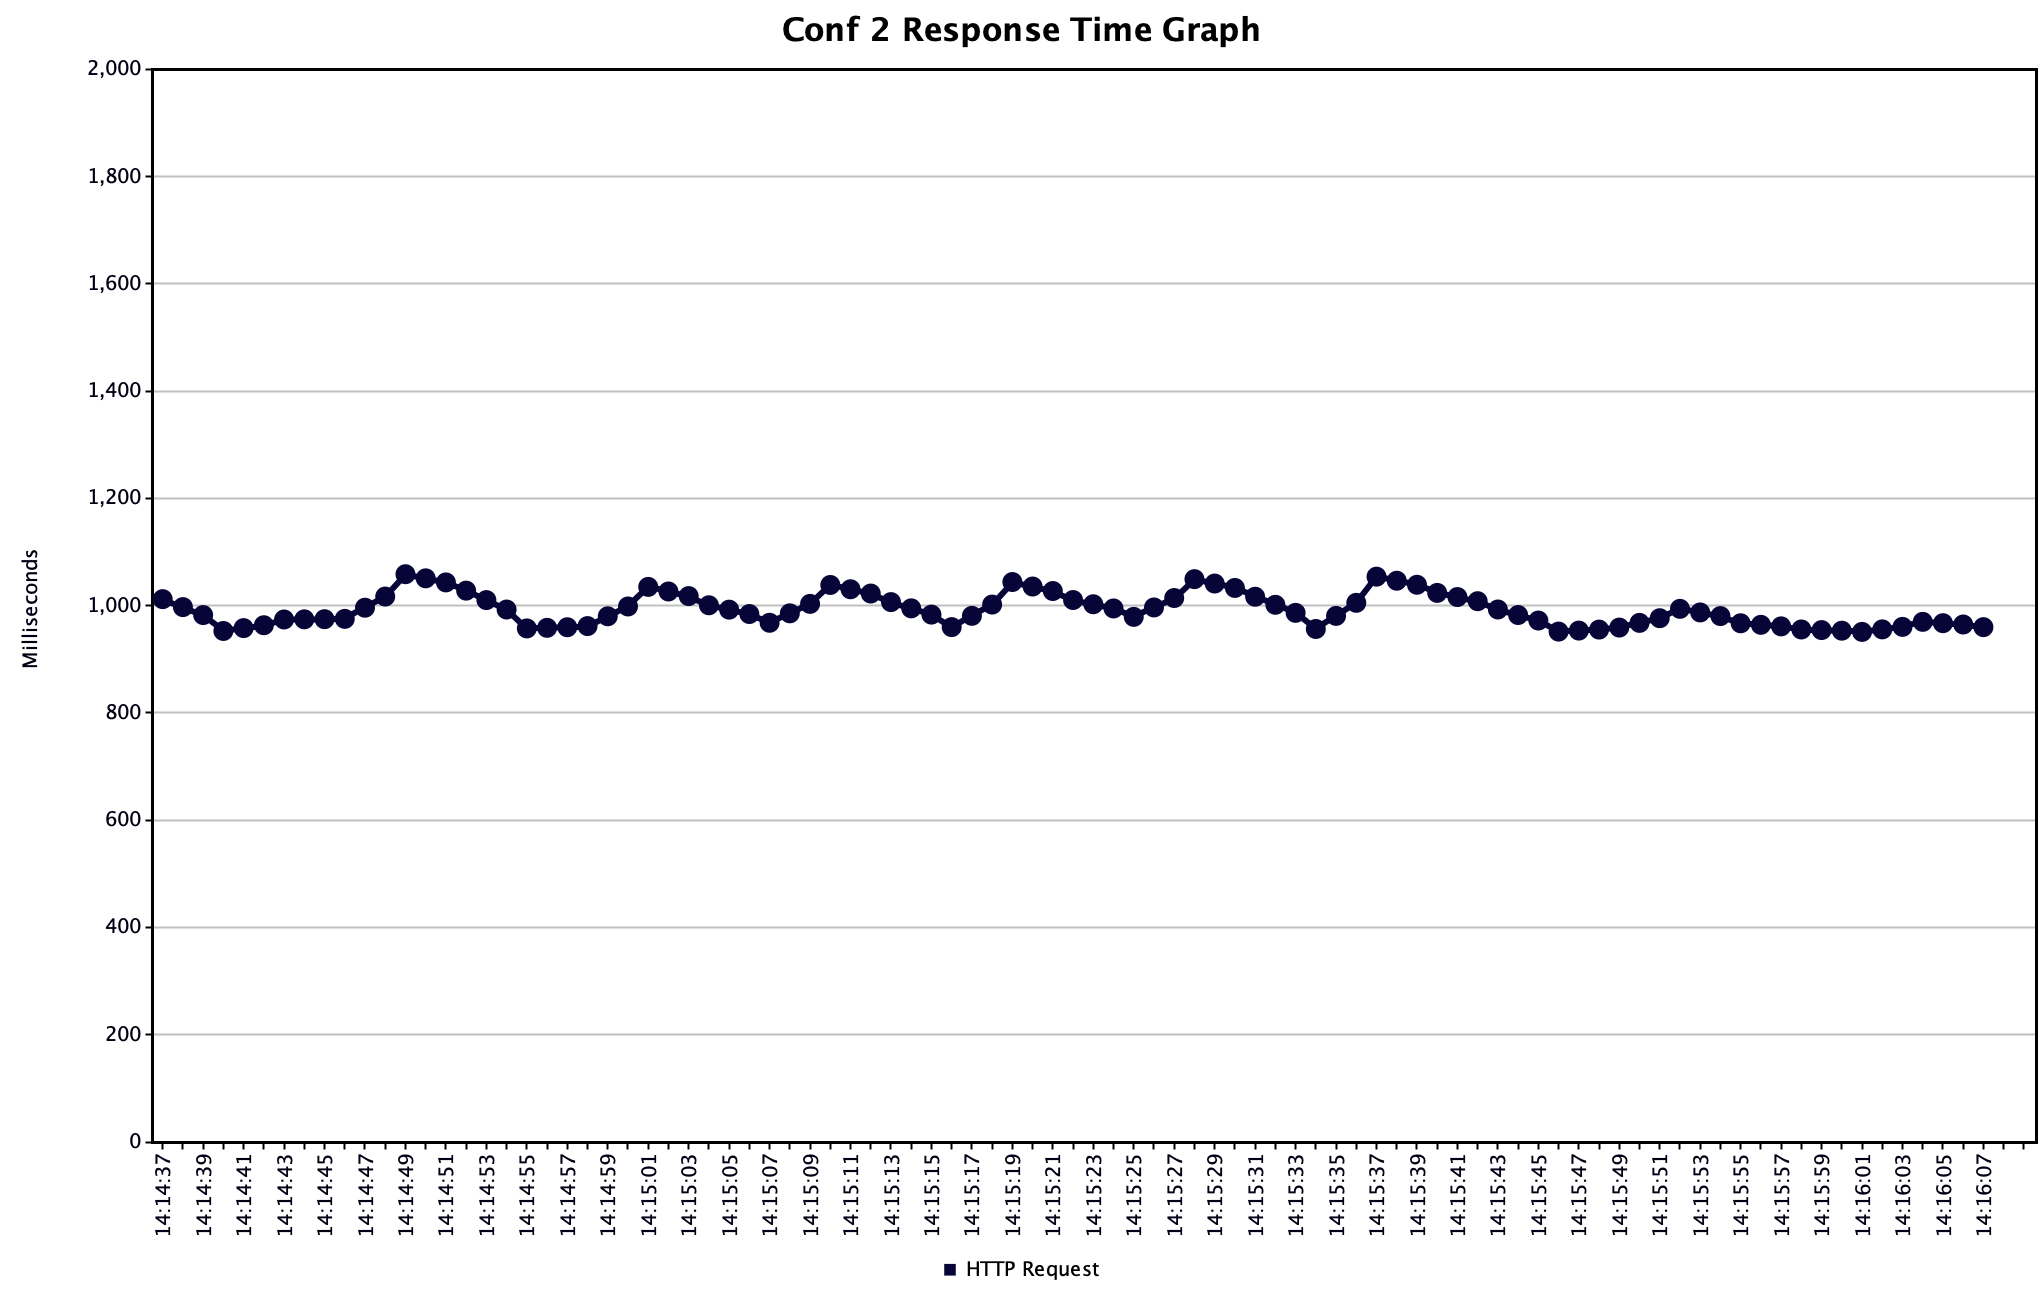
\includegraphics[width=\textwidth]{image/resp-graph-conf-2.png}
  \caption{График пропускной способности для конфигурации 2}
\end{figure}

\begin{figure}[H]
  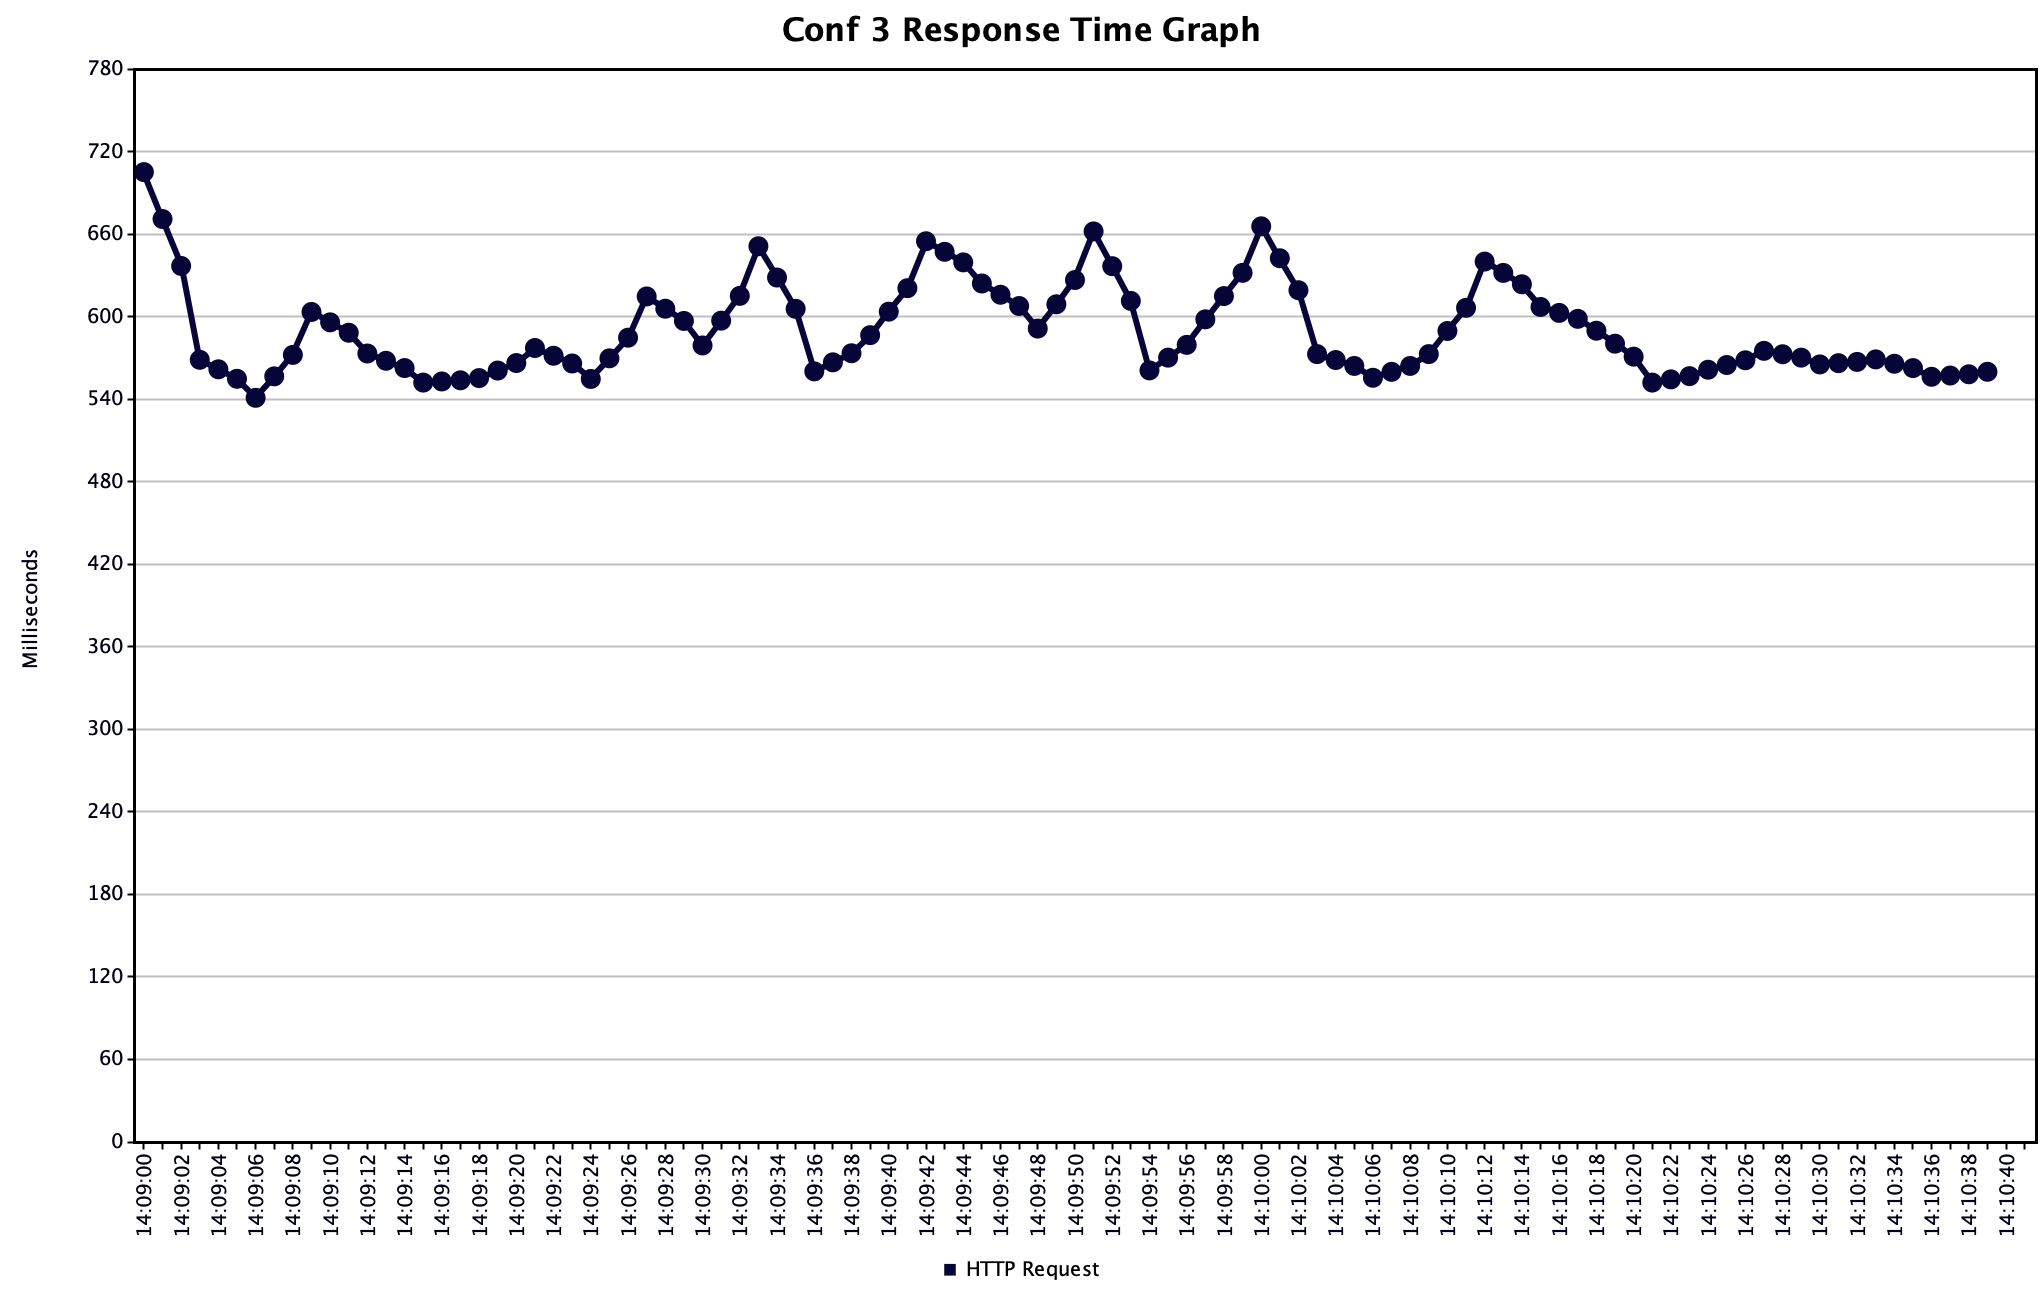
\includegraphics[width=\textwidth]{image/resp-graph-conf-3.png}
  \caption{График пропускной способности для конфигурации 3}
\end{figure}

\begin{figure}[H]
  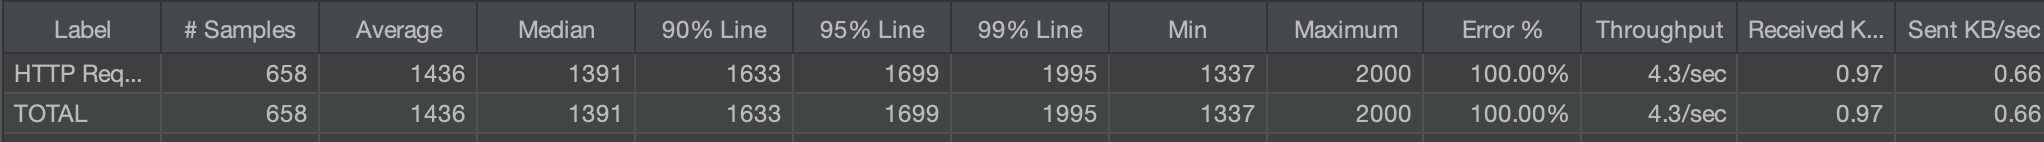
\includegraphics[width=\textwidth]{image/aggregate-report-conf1.png}
  \caption{Агрегированный отчёт для конфигурации 1}
\end{figure}

\begin{figure}[H]
  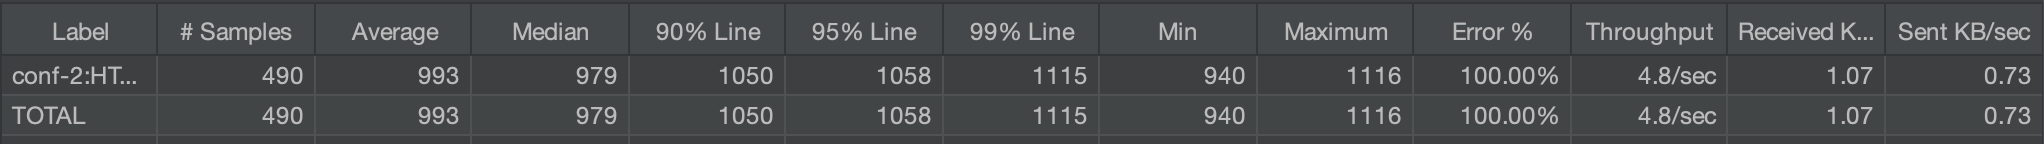
\includegraphics[width=\textwidth]{image/aggregate-report-conf2.png}
  \caption{Агрегированный отчёт для конфигурации 2}
\end{figure}

\begin{figure}[H]
  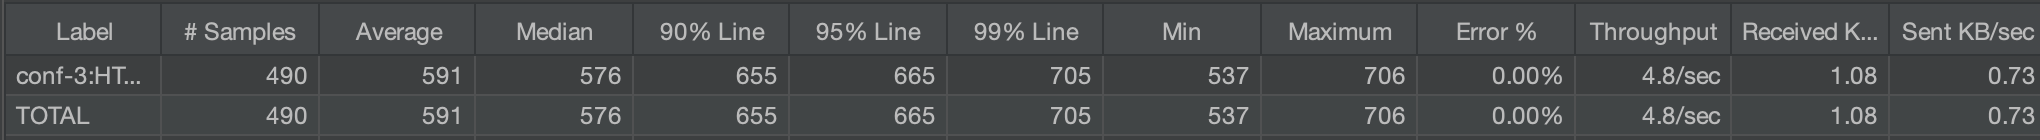
\includegraphics[width=\textwidth]{image/aggregate-report-conf3.png}
  \caption{Агрегированный отчёт для конфигурации 3}
\end{figure}



Мы видим, что конфигурации 1 и 2 не проходят порог максимального допустимого времени обработки.
Для них 95 процентиль среднего равен 1699 и 1050 соответсвенно, тогда как требуется менее 920 мс.

Третья конфигурация удовлетворяет требованиям по времени обработки запроса, так как 95 процентиль равен 665 мс.

\section*{Описание конфигурации JMeter для стресс-тестирования.}
\begin{figure}[H]
  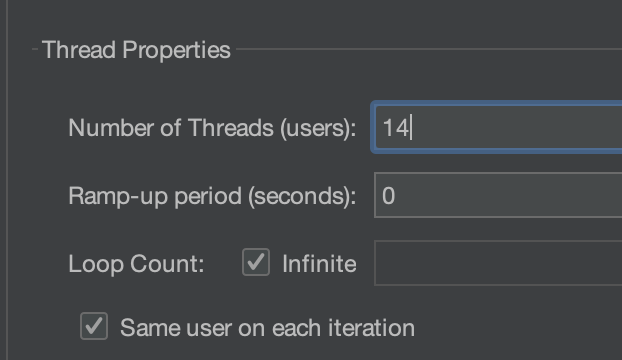
\includegraphics[width=\textwidth]{image/conf-stress.png}
  \caption{Вид конфигурации для стресс-тестирования}
\end{figure}
\begin{figure}[H]
  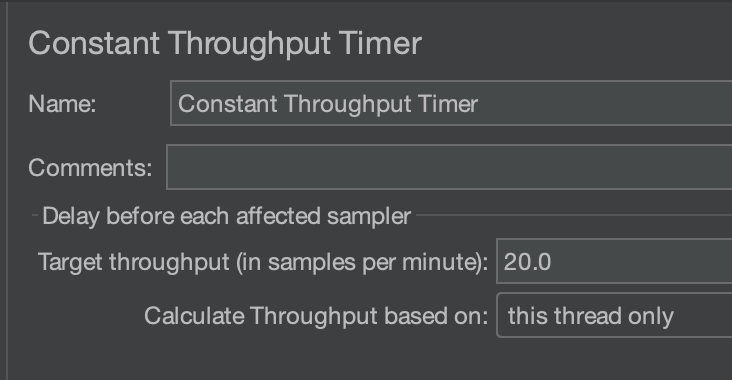
\includegraphics[width=\textwidth]{image/throughput-timer-stress.png}
  \caption{Вид конфигурации для стресс-тестирования}
\end{figure}

\section*{График изменения времени отклика от нагрузки для выбранной конфигурации, полученный в ходе стресс-тестирования системы.}
\begin{figure}[H]
  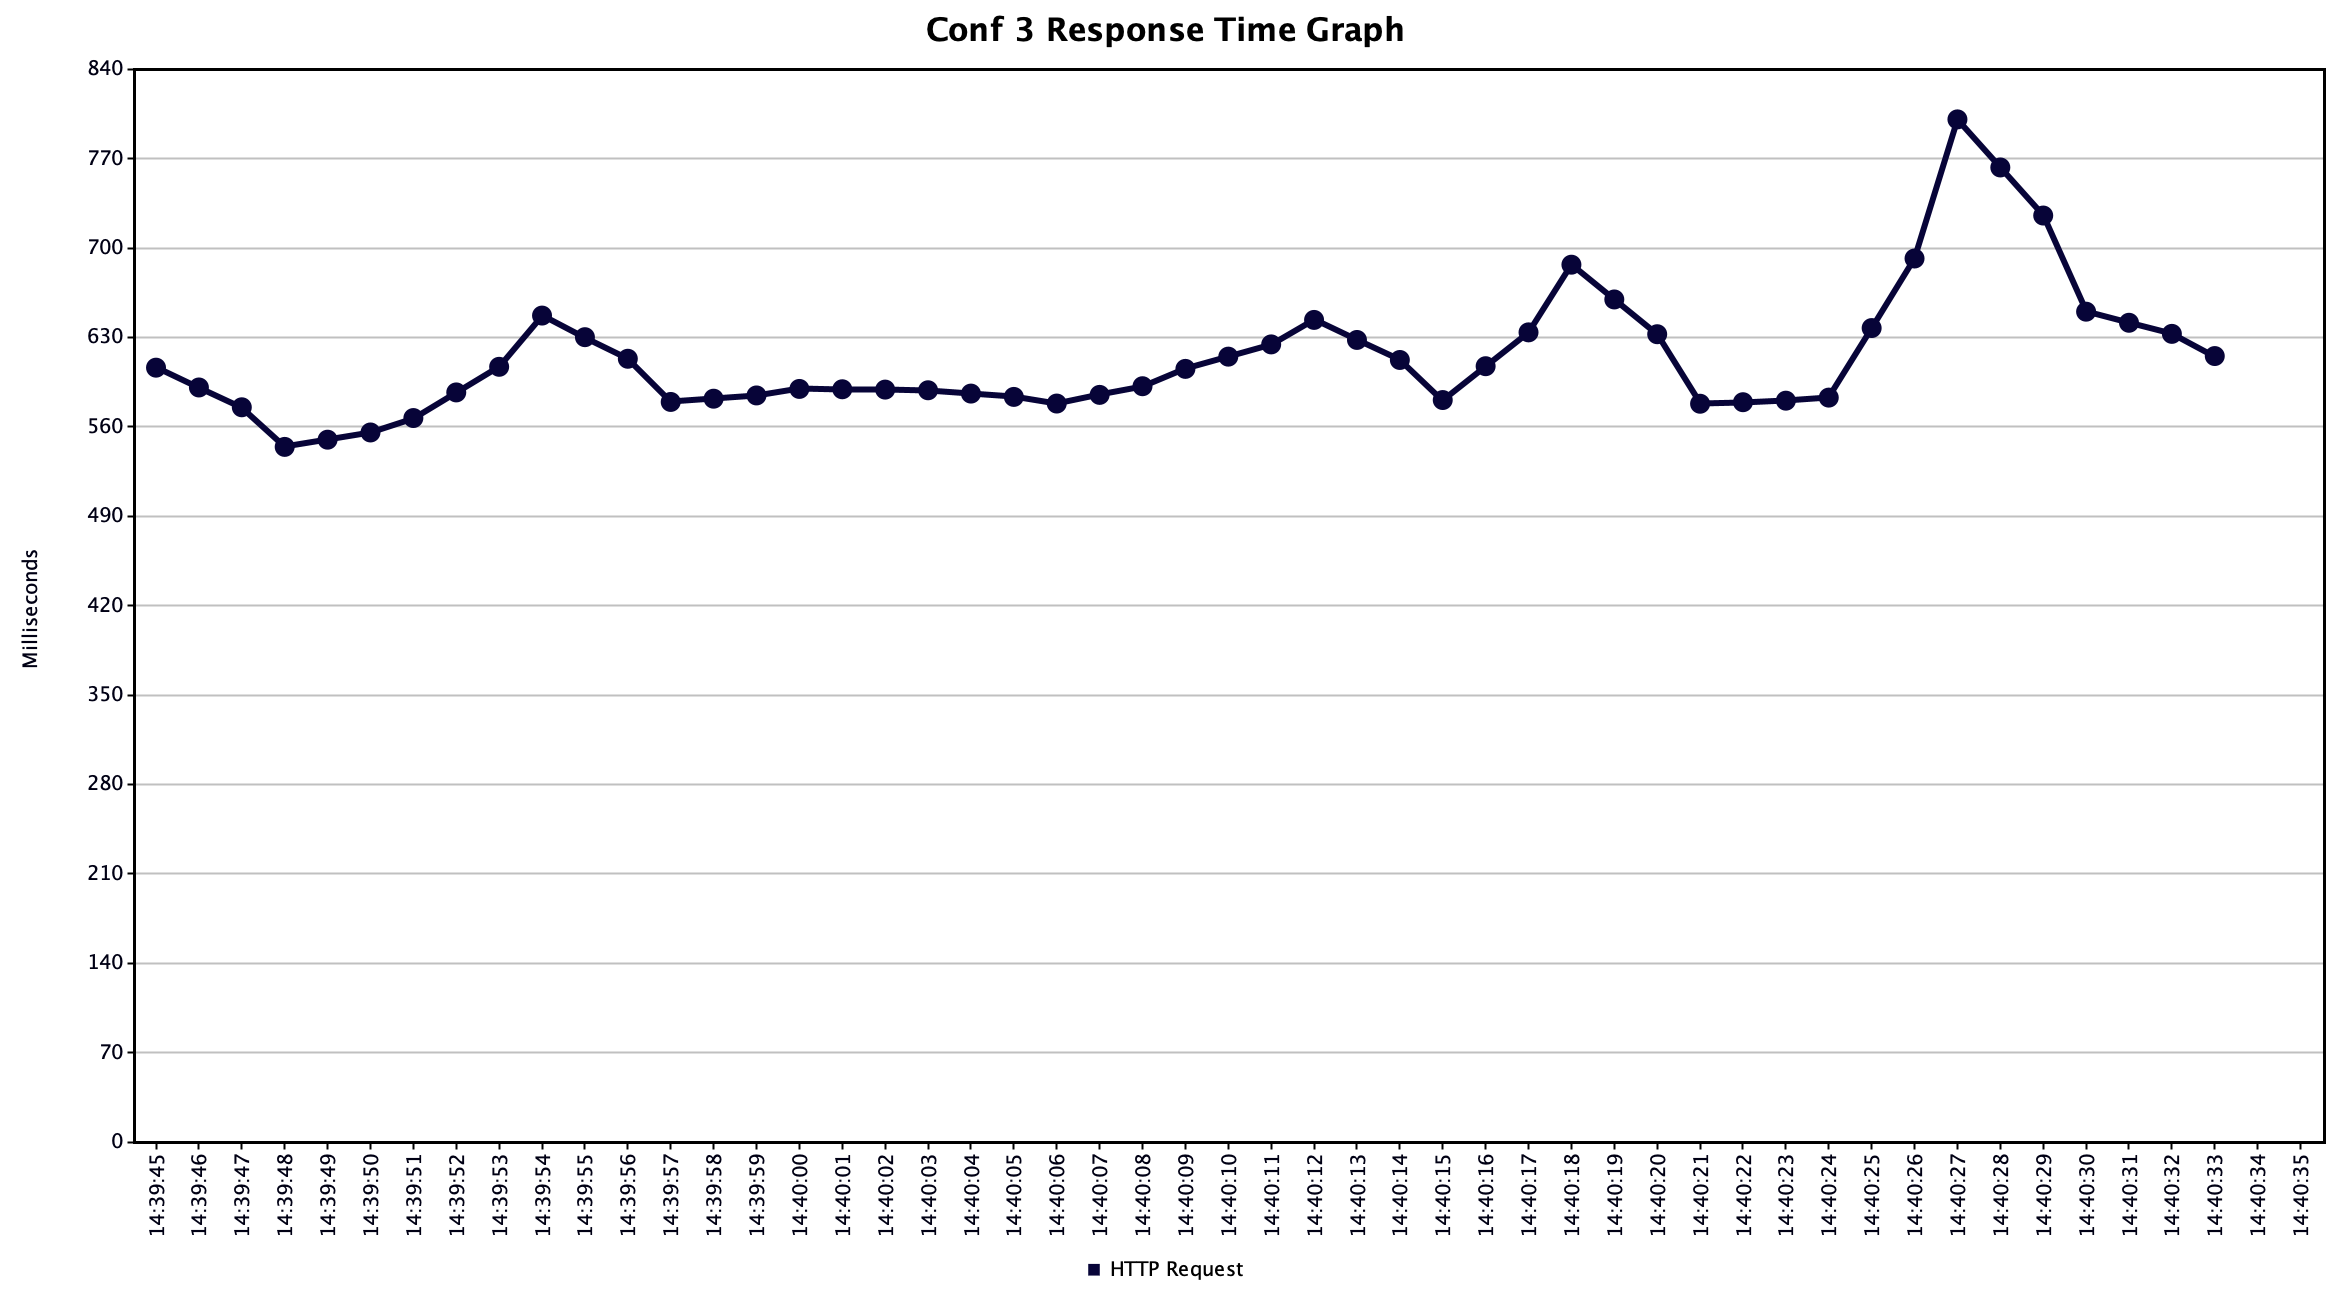
\includegraphics[width=\textwidth]{image/resp-graph-conf-3-2.png}
  \caption{График изменения времени отклика при нагрузке в 20 пользователей}
\end{figure}

Видим, что при 20 пользователях время отклика не превышает 920 мс.

\begin{figure}[H]
  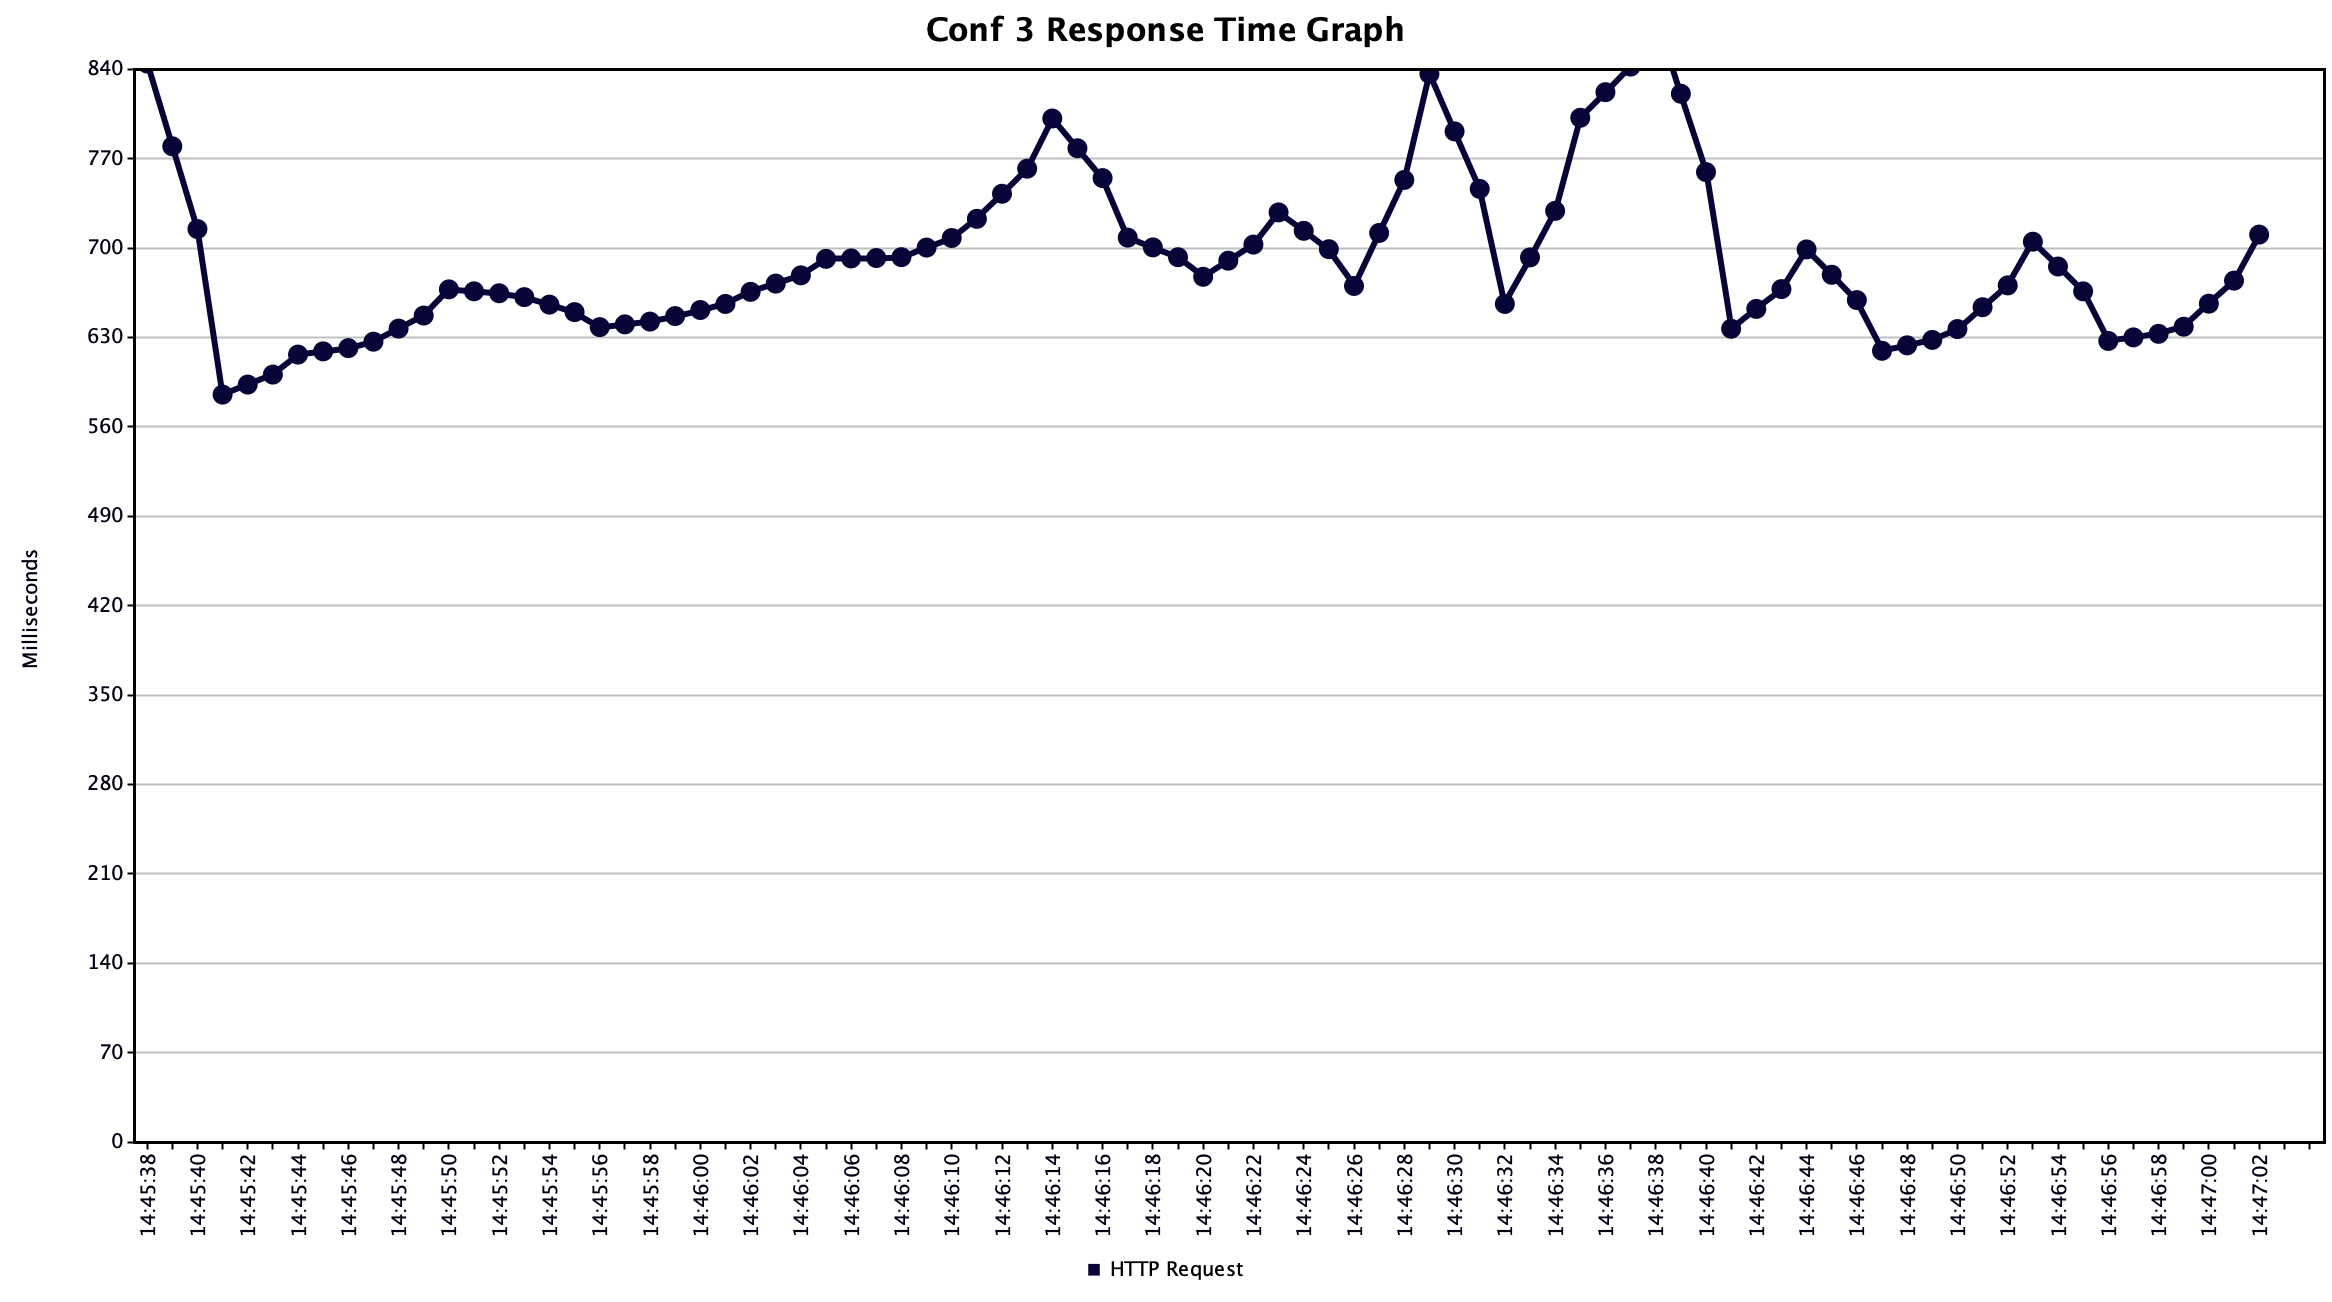
\includegraphics[width=\textwidth]{image/resp-graph-conf-3-3.png}
  \caption{График изменения времени отклика при нагрузке в 30 пользователей}
\end{figure}

\begin{figure}[H]
  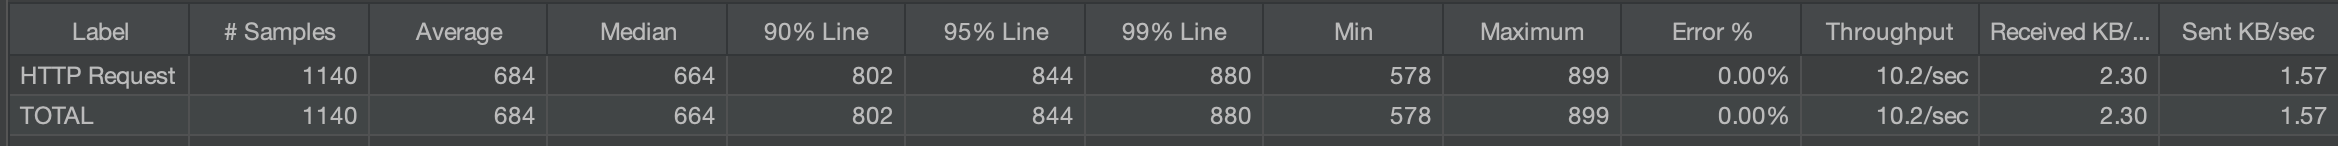
\includegraphics[width=\textwidth]{image/aggregate-report-conf3-3.png}
  \caption{Агрегированный отчёт при нагрузке в 30 пользователей}
\end{figure}

Видим, что время отклика увеличилось, но всё ещё не превышает 920 мс.

\begin{figure}[H]
  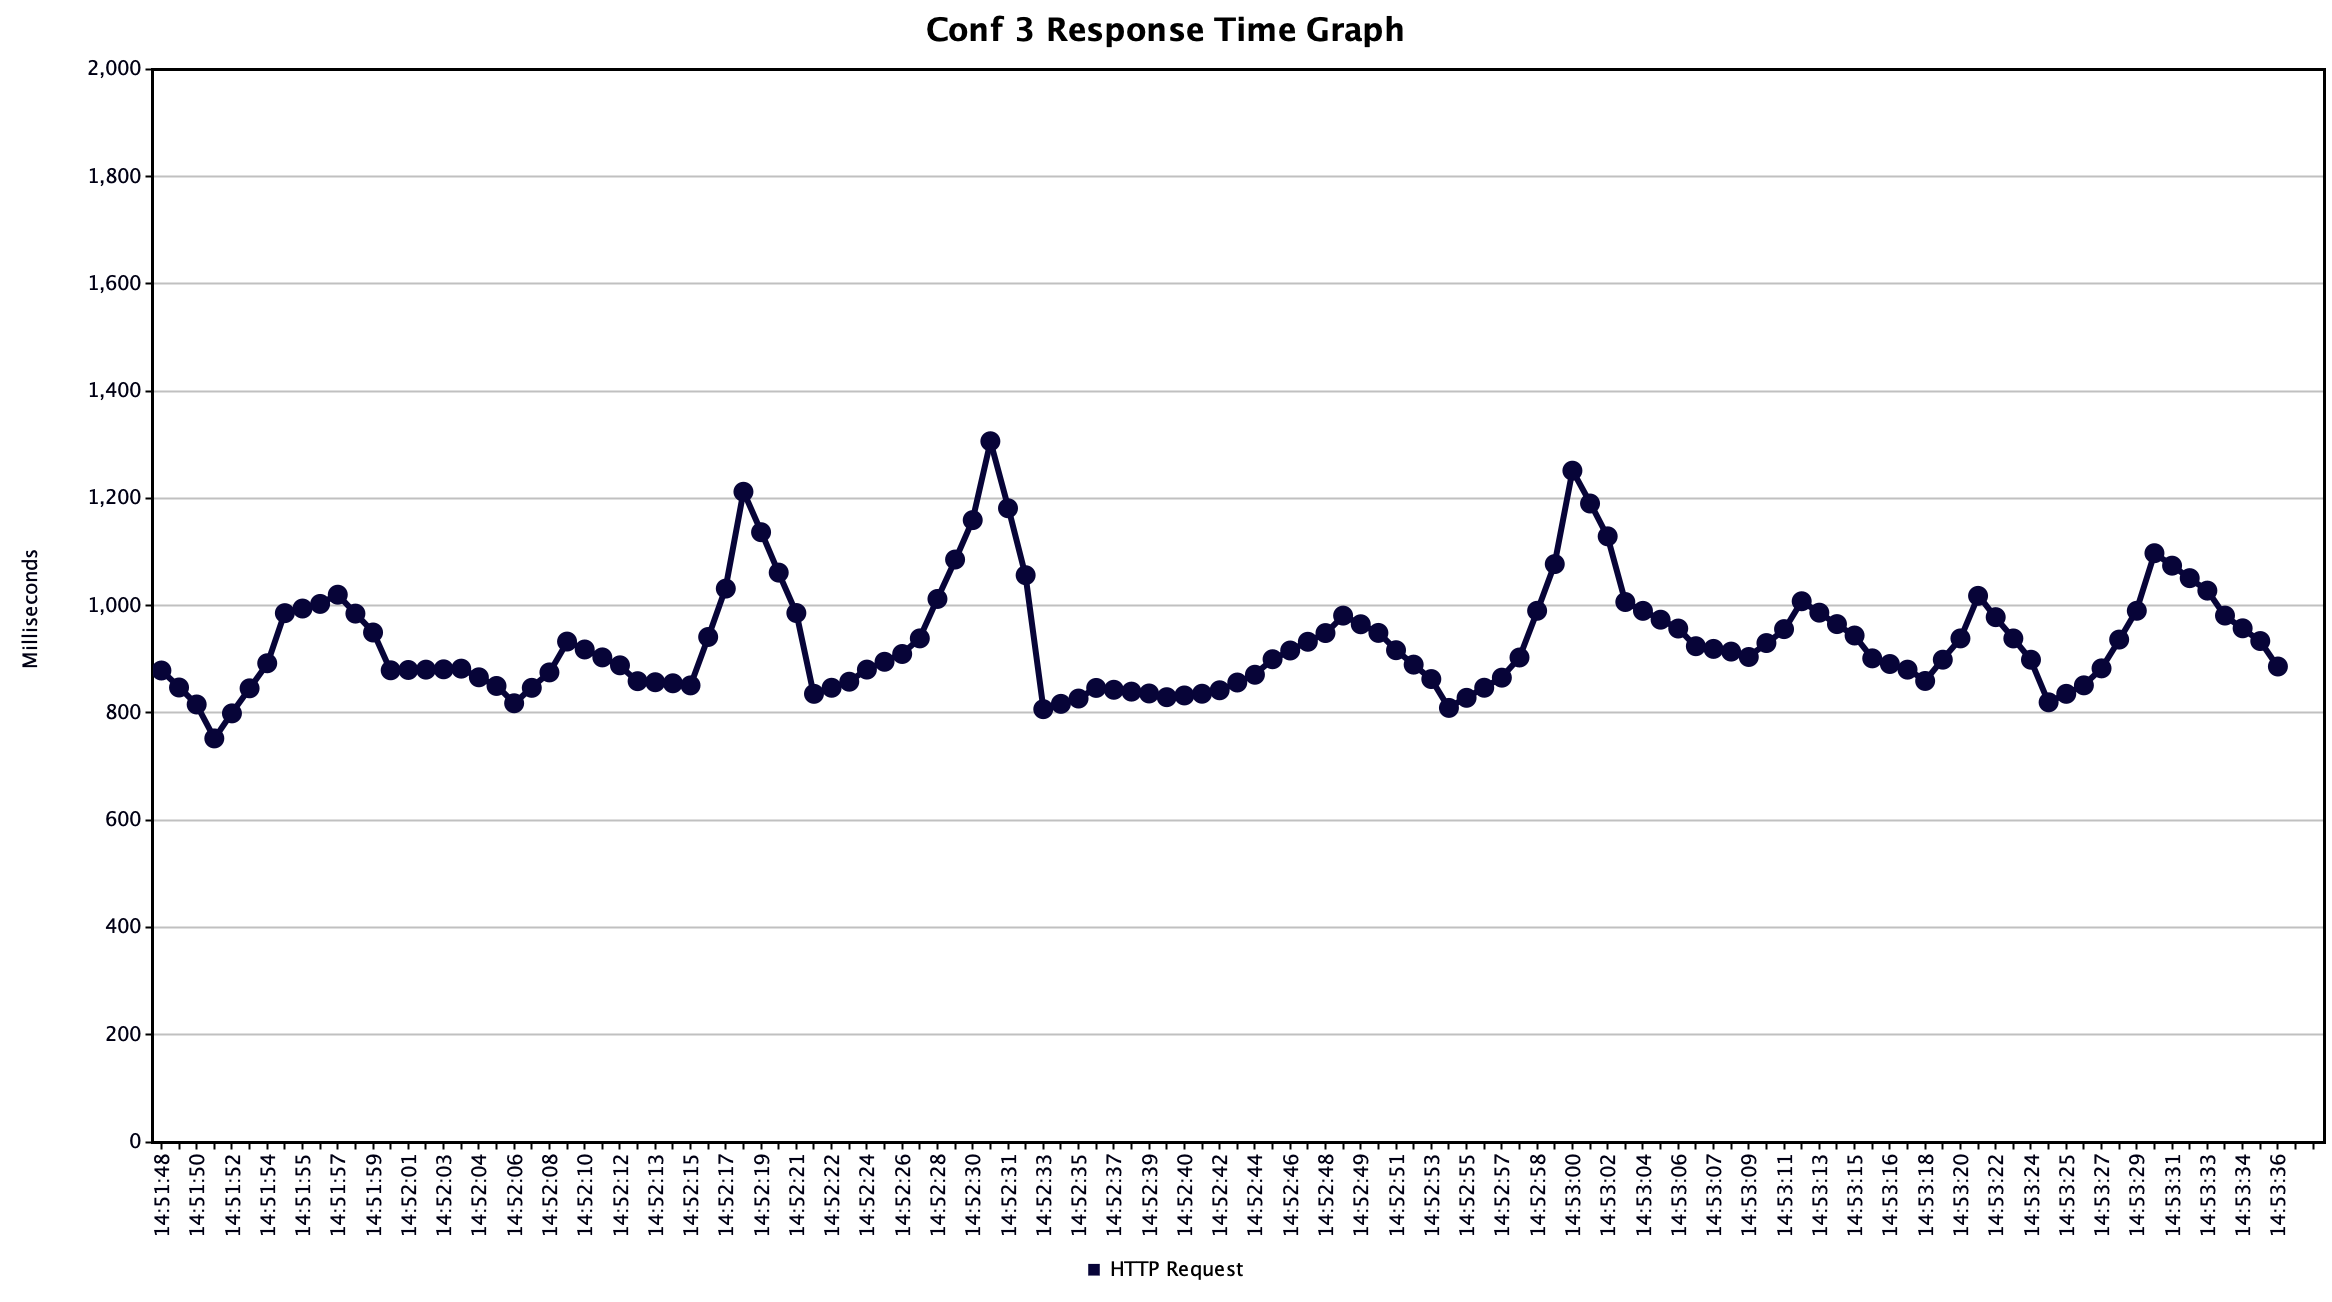
\includegraphics[width=\textwidth]{image/resp-graph-conf-3-4.png}
  \caption{График изменения времени отклика при нагрузке в 40 пользователей}
\end{figure}

\begin{figure}[H]
  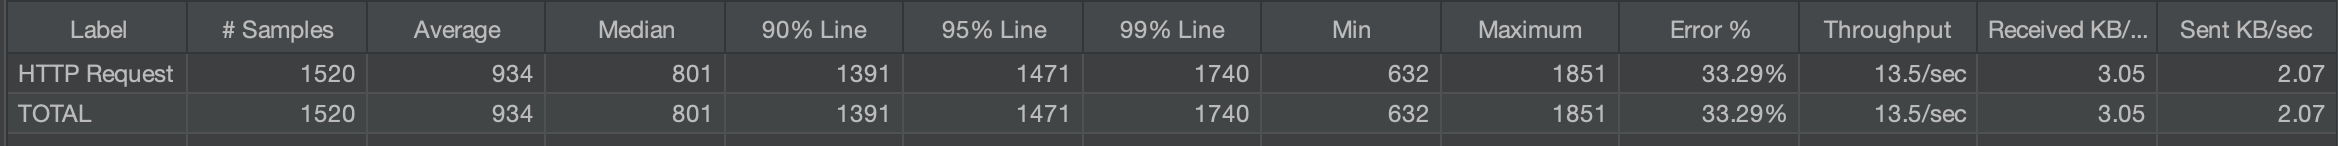
\includegraphics[width=\textwidth]{image/aggregate-report-conf3-4.png}
  \caption{Агрегированный отчёт при нагрузке в 40 пользователей}
\end{figure}

Видим, что время отклика увелисилось и некоторые запросы превышают 920 мс.
Процент запросов, которые превышают 920 мс равен 33.29 процентов.

При нагрузке в 35 пользователей, процент запросов, которые превышают 920 мс равен 8.75 процентов.

При нагрузке в 32 пользователей, процент запросов, которые превышают 920 мс равен 2.03 процентов.

При нагрузке в 31 пользователей, процент запросов, которые превышают 920 мс равен 1.36 процентов.

Таким образразом пороговое значение числа потоков равно 30.

\begin{figure}[H]
  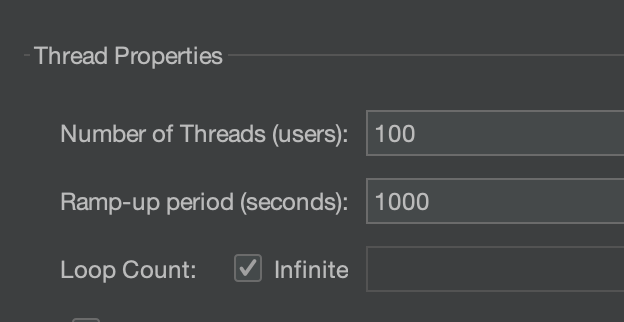
\includegraphics[width=\textwidth]{image/final-conf.png}
  \caption{Конфигурация для стресс-тестирования}
\end{figure}
Увеличиваем количество потоков от 1 до 1000 каждые 10 секунд.
\begin{figure}[H]
  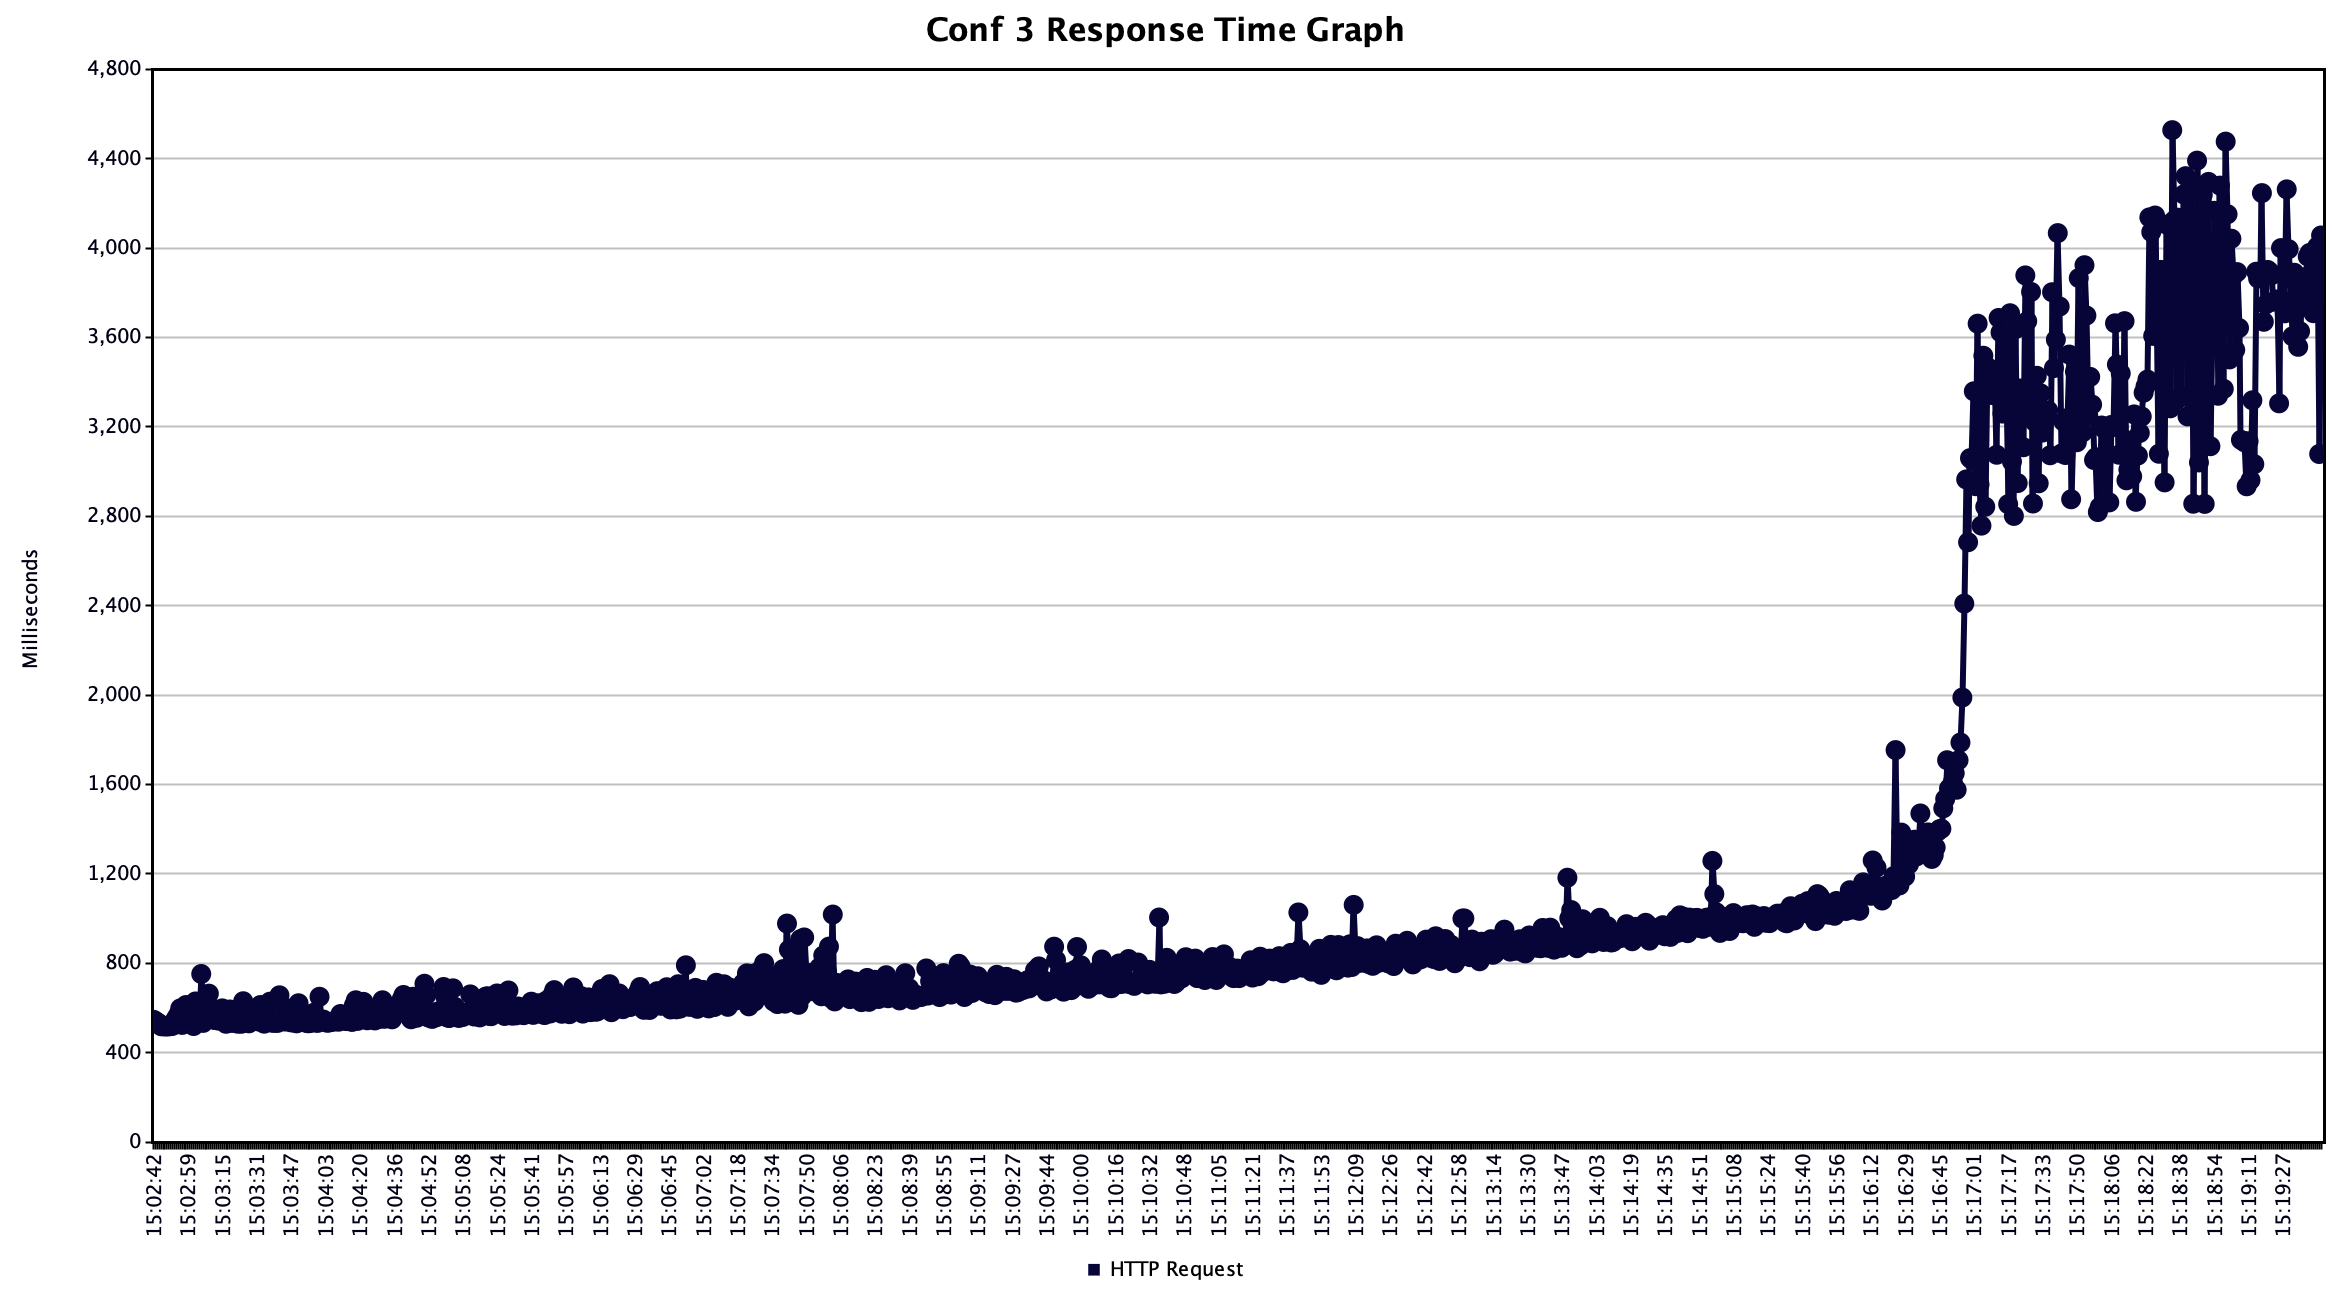
\includegraphics[width=\textwidth]{image/resp-time-graph.png}
  \caption{График зависимости времени отклика от нагрузки}
\end{figure}

Заметим, что после 85 пользователей время отклика начинает резко увеличиваться.
Таким образом ~80 пользователей - это максимальная нагрузка для данного сервера. 





\section*{Выводы по работе.}
В процессе выполнения данной лабораторной работы я познакомился с
инструментом Apache JMeter, который используется для проведения нагрузочного тестирования. С
его помощью я провёл нагрузочное тестирование 3 различных конфигураций, выданных по
варианту, и определил, что заданным условиям максимального времени отклика удовлетворяет
только конфигурация Nº3. После этого я провёл стресс-тестирование этой конфигурации и
выявил, что максимальная нагрузка, при которой время ожидания ответа не будет выходить за
рамки 920мс, составляет 30 одновременных пользователей.
\end{document}